\documentclass[conference]{IEEEtran}
\usepackage{amsmath,amssymb,amsfonts}
\usepackage{amsthm}
\newtheorem{proposition}{Proposition}
\usepackage{graphicx}
\usepackage{float}
\usepackage{pifont}
\usepackage{xcolor}
\usepackage{url}
\usepackage{textcomp}
\usepackage{tikz}
\usetikzlibrary{arrows.meta,positioning,calc,backgrounds,fit,shadows}
\graphicspath{{figures/}}
\newcommand{\VRMSE}{20.3}
\newcommand{\VRMSEho}{21.3}
\newcommand{\TRMSE}{1.32}
\newcommand{\platRMSE}{8.2}
\newcommand{\platMargin}{19.0}
\newcommand{\platMarginMax}{38.9}
\newcommand{\oursWarmEta}{86.53}
\newcommand{\oursWarmSoc}{0.773}
\newcommand{\cctwoWarmEta}{84.40}
\newcommand{\cconeWarmSoc}{0.773}
\newcommand{\cconeWarmEta}{87.85}
\newcommand{\offWarmSoc}{0.798}
\newcommand{\offWarmEta}{85.88}
\newcommand{\oursWarmDL}{0}
\newcommand{\oursWarmTime}{nan}
\newcommand{\cconeWarmDL}{0}
\newcommand{\cctwoWarmTime}{24.3}
\newcommand{\oursColdEta}{86.95}
\newcommand{\oursColdSoc}{0.707}
\newcommand{\cctwoColdEta}{84.10}
\newcommand{\cconeColdSoc}{0.765}
\newcommand{\cconeColdEta}{87.32}
\newcommand{\offColdSoc}{0.798}
\newcommand{\offColdEta}{86.24}
\newcommand{\oursColdDL}{0}
\newcommand{\oursColdTime}{nan}
\newcommand{\cconeColdDL}{0}
\newcommand{\cctwoColdTime}{26.3}
\newcommand{\cctwoWarmTviol}{100.0}
\newcommand{\cctwoWarmPviol}{100.0}
\newcommand{\ppotimeWarmviol}{0.0}
\newcommand{\ppolagWarmviol}{14.4}
\newcommand{\oursWarmN}{500}
\newcommand{\oursWarmUpper}{0.60}
\newcommand{\cctwoColdTviol}{0.0}
\newcommand{\cctwoColdPviol}{100.0}
\newcommand{\ppotimeColdviol}{0.0}
\newcommand{\ppolagColdviol}{0.0}
\newcommand{\oursColdN}{60}
\newcommand{\oursColdUpper}{4.87}
\newcommand{\optgapWarm}{0.49}
\newcommand{\oursIQMWarm}{85.59}
\newcommand{\optgapCold}{-1.03}
\newcommand{\oursIQMCold}{86.87}
\newcommand{\agingOursViol}{0.0}
\newcommand{\agingPPOLagViol}{83.3}
\newcommand{\agingSoftViol}{0.0}
\newcommand{\agingFixnomViol}{100.0}
\newcommand{\agingOursViolFresh}{0.0}
\newcommand{\agingPPOLagViolFresh}{15.8}
\newcommand{\agingSoftViolFresh}{0.0}
\newcommand{\agingFixnomViolFresh}{0.0}
\newcommand{\ccHalfColdSoc}{0.452}
\newcommand{\refgovWarmSoc}{0.773}
\newcommand{\refgovWarmEta}{86.49}
\newcommand{\ccHalfWarmSoc}{0.446}
\newcommand{\ccHalfWarmEta}{85.59}
\newcommand{\cconeWarmPviol}{22}
\newcommand{\mpcnomWarmSoc}{0.782}
\newcommand{\sohErrViol}{0.0}
\newcommand{\sohErrViolMarg}{0.0}
\newcommand{\dfnPlatePerturbRate}{0}
\newcommand{\qpMainN}{100}
\newcommand{\qpCornerN}{50}
\newcommand{\qpFullIterMeanMild}{37}
\newcommand{\qpFullIterMaxMild}{550}
\newcommand{\qpFullIterMean}{85}
\newcommand{\qpFullIterMax}{775}
\newcommand{\qpEmbNonconv}{100}
\newcommand{\qpEmbWorstV}{4.186}
\newcommand{\qpFilterWorstV}{4.181}
\newcommand{\gainSafeCells}{15}
\newcommand{\gainCells}{15}
\newcommand{\coolSafeLoss}{33}
\newcommand{\transferErrT}{0.42}
\newcommand{\priceTotal}{1.3}
\newcommand{\priceThermal}{0.2}
\newcommand{\priceBinder}{1.4}
\newcommand{\dimEnvChan}{5}
\newcommand{\dimEnvN}{50000}
\newcommand{\dimEnvCP}{0.006}
\newcommand{\dimEnvWorstT}{44.5}
\newcommand{\dimCertIters}{18}
\newcommand{\filterSloc}{36}
\newcommand{\qpTcbFiles}{39}
\newcommand{\qpTcbMb}{1.1}
\newcommand{\mpcNomViol}{100}
\newcommand{\mpcNomMs}{176}
\newcommand{\mpcNomEta}{87.3}
\newcommand{\mpcNomSoc}{0.785}
\newcommand{\mpcOracleViol}{0}
\newcommand{\mpcOracleMs}{121}
\newcommand{\mpcOracleEta}{87.4}
\newcommand{\mpcOracleSoc}{0.779}
\newcommand{\mpcBoundedViol}{0}
\newcommand{\mpcBoundedMs}{148}
\newcommand{\mpcBoundedEta}{87.4}
\newcommand{\mpcBoundedSoc}{0.779}
\newcommand{\mpcOursViol}{0}
\newcommand{\mpcOursMs}{0}
\newcommand{\mpcOursEta}{86.7}
\newcommand{\mpcOursSoc}{0.724}
\newcommand{\dfnOursColdSurf}{10.8}
\newcommand{\dfnOursColdT}{26.3}
\newcommand{\dfnCctwoColdSurf}{-62.2}
\newcommand{\dfnCctwoColdT}{41.8}
\newcommand{\dfnOursWarmSurf}{13.2}
\newcommand{\dfnOursWarmT}{40.4}
\newcommand{\dfnCctwoWarmSurf}{-3.1}
\newcommand{\dfnCctwoWarmT}{52.8}
\newcommand{\platMonoSlope}{5.3}
\newcommand{\platMonoPmin}{5.3}
\newcommand{\platMonoCorner}{-0.30}
\newcommand{\oodTotN}{200}
\newcommand{\oodTotSafe}{196}
\newcommand{\oodWorst}{-2.0}
\newcommand{\oodWarmSafe}{99}
\newcommand{\oodWarmN}{100}
\newcommand{\oodColdSafe}{97}
\newcommand{\oodColdN}{100}
\newcommand{\oodColdCP}{7.6}
\newcommand{\oodTotCP}{4.5}
\newcommand{\estViolMax}{0.0}
\newcommand{\estViolNoise}{0.0}
\newcommand{\nomAgedViol}{100}
\newcommand{\estNforSOH}{288}
\newcommand{\estSocFresh}{0.772}
\newcommand{\estSocAged}{0.589}
\newcommand{\estNomSocAged}{0.781}
\newcommand{\estRestAged}{1.77}
\newcommand{\clSocAged}{0.563}
\newcommand{\clPeakTAged}{35.9}
\newcommand{\clRestAged}{1.44}
\newcommand{\clRtrueAged}{1.80}
\newcommand{\clNomSocAged}{0.765}
\newcommand{\clNomPeakTAged}{41.3}
\newcommand{\clOracleSocAged}{0.533}
\newcommand{\clSocMid}{0.776}
\newcommand{\clPeakTMid}{40.9}
\newcommand{\crossChenSafe}{2}
\newcommand{\crossChenN}{2}
\newcommand{\crossChenT}{40.6}
\newcommand{\crossChenV}{4.17}
\newcommand{\crossEnsSafe}{60}
\newcommand{\crossEnsN}{60}
\newcommand{\crossEnsT}{36.1}
\newcommand{\crossEnsV}{4.16}
\newcommand{\crossEnsCP}{4.9}
\newcommand{\precondHiSR}{1.80}
\newcommand{\precondHiT}{30.1}
\newcommand{\precondDipMin}{29}
\newcommand{\precondDipI}{0.7}
\newcommand{\precondDipHead}{13.8}
\newcommand{\precondDipT}{31.2}
\newcommand{\boundThermAged}{6.8}
\newcommand{\boundThermErrAged}{7.3}
\newcommand{\boundPlateFresh}{13.5}
\newcommand{\boundPlateAged}{42.3}
\newcommand{\jointSafe}{78}
\newcommand{\jointN}{78}
\newcommand{\jointWorstT}{40.4}
\newcommand{\agedDfnSafe}{40}
\newcommand{\agedDfnN}{40}
\newcommand{\agedDfnWorstT}{39.3}
\newcommand{\agedDfnWorstPlate}{6.1}
\newcommand{\valSafe}{156}
\newcommand{\valN}{156}
\newcommand{\valWorstT}{41.9}
\newcommand{\aggSafe}{196}
\newcommand{\aggN}{196}
\newcommand{\aggWorstT}{41.9}
\newcommand{\aggCP}{1.5}
\newcommand{\valCP}{1.9}
\newcommand{\filterMs}{0.87}
\newcommand{\coreWorstHi}{45.1}
\newcommand{\coreWorstLo}{43.1}
\newcommand{\gradHi}{6.2}
\newcommand{\gradLo}{3.9}
\newcommand{\kReserve}{0.74}
\newcommand{\reserveDT}{4.2}
\newcommand{\coreSocLo}{0.728}
\newcommand{\coreSocHi}{0.663}
\newcommand{\coreCostLo}{4.4}
\newcommand{\coreCostHi}{10.9}
\newcommand{\chemTwoV}{26.5}
\newcommand{\chemTwoT}{0.12}
\newcommand{\chemTwoSafe}{100}
\newcommand{\chemTwoN}{100}
\newcommand{\chemTwoWorstT}{28.1}
\newcommand{\chemTwoWorstV}{4.20}
\newcommand{\chemTwoCP}{3.0}
\newcommand{\chemTwoQ}{2.28}
\newcommand{\irrevPlateWarm}{18.9}
\newcommand{\irrevPlateCold}{13.0}
\newcommand{\jointCP}{3.8}
\newcommand{\jointNbig}{78}
\newcommand{\estSocD}{0.678}
\newcommand{\worstRSocD}{0.360}
\newcommand{\coTwoSavedPerCharge}{1412.0}
\newcommand{\coTwoFracSaved}{1.88}
\newcommand{\coTwoLo}{42}
\newcommand{\coTwoHi}{1059}
\newcommand{\platCP}{6.7}
\newcommand{\platNbig}{80}
\newcommand{\platViolBig}{1}

%% --- added for the IECON revision: reviewer-requested quantities ---
%% Prop. 2 monotonicity (reproduce/ + tests/test_safety.py)
\newcommand{\revFrac}{24}          % max |Q_rev|/Q_irr over the admissible 0.7C-2C band [%]
\newcommand{\monoImin}{0.08}       % dI g_T >= 0 for all I above this C-rate
\newcommand{\platCapFloor}{0.70}   % floor of the temperature-dependent plating cap [C]
%% Control step (reproduce/step_size.py)
\newcommand{\stepLo}{5}            % shortest control step tested [s]
\newcommand{\stepHi}{120}          % longest control step tested [s]
\newcommand{\rcResidPct}{10}       % worst RC residual as a fraction of the base margin [%]
\newcommand{\stepSocSpread}{0.1}   % spread in delivered SOC across the step sweep [points]
%% Bisection tolerance (reproduce/tolerance_sweep.py)
\newcommand{\tolIters}{18}
\newcommand{\tolEpsUA}{38}         % current resolution at 18 iterations [uA]
\newcommand{\tolKnee}{12}          % iterations beyond which delivered charge saturates
%% Real-time cost (bench/timing.py)
\newcommand{\filterEvalMax}{20}    % model evaluations per projection, hard bound
\newcommand{\filterMeanUs}{56}     % full-bisection path, median per projection [us] (bench/timing.py)
\newcommand{\filterFlops}{800}
\newcommand{\filterMemB}{904}      % state + constants, double precision [B]
%% Robustness beyond the bound (reproduce/robustness.py)
\newcommand{\eolBreakSR}{3.0}      % first violation as the true resistance scale is raised
\newcommand{\eolBreakX}{1.7}       % ... as a multiple of the rated bound
\newcommand{\gainGrid}{273}         % gain settings swept
\newcommand{\gainRuns}{27027}       % gain settings x aged cooling-faulted cells

\newcommand{\iecomainrows}{%
CC--CV 1C & 87.8 & 0.773 & 38.7 & 22\\
CC--CV 2C & 84.4 & 0.803 & 53.5 & 100\\
MSCC & 85.0 & 0.802 & 50.5 & 100\\
Offline opt. & 85.9 & 0.798 & 44.5 & 0\\
PPO-Lag (no filter) & 87.3 & 0.734 & 40.1 & 9\\
\textbf{Ours} & 86.5 & 0.773 & 40.7 & $\le$0.60\\
}

\newcommand{\safetytablerows}{%
Fresh cell, $T$/$V$ (warm) & 500 & 0 & $\le$0.6\\
Aged $T$/$V$, disjoint held-out & 156 & 0 & $\le$1.9\\
Aged $T$/$V$, pooled & 196 & 0 & $\le$1.5\\
Joint noise$+$aging$+$DFN & 78 & 0 & $\le$3.8\\
Cross-param.\ aged $T$/$V$ (Chen \emph{et al.}) & 60 & 0 & $\le$4.9\\
2nd chemistry, recalibrated (Ai \emph{et al.}) & 100 & 0 & $\le$3.0\\
}
 % consolidated (test, n, violations, CP bound) rows
% ROM param table body
\newcommand{\romparamrows}{%
Nominal capacity $Q_\mathrm{nom}$ & 5.00 & Ah\\
Ohmic activation $E_a/R$ & 2435 & K\\
RC time constant $\tau_1$ & 30 & s\\
Lumped heat capacity $C_\mathrm{th}$ & 101.6 & J/K\\
Heat-transfer coeff.\ $hA$ & 0.0799 & W/K\\
Entropic coeff.\ $dU/dT$ & -0.112 & mV/K\\
Plating margin $\phi_\mathrm{marg}$ & 19.0 & mV\\
}

\newcommand{\calibrows}{%
Voltage RMSE (train / hold-out) & 20.3 / 21.3 & mV\\
Voltage max err (hold-out) & 51.8 & mV\\
Temperature RMSE (train / hold-out) & 1.32 / 1.44 & \degC\\
Plating-potential RMSE & 8.2 & mV\\
}

\newcommand{\estoraclerows}{%
1.00 & 0 & 0.772 & 1.00 & 1.00 & 25.0\\
0.95 & 0 & 0.751 & 1.00 & 1.20 & 25.0\\
0.90 & 0 & 0.712 & 1.00 & 1.40 & 25.0\\
0.85 & 0 & 0.637 & 1.00 & 1.60 & 26.6\\
0.80 & 0 & 0.542 & 1.00 & 1.80 & 36.6\\
}

% NOTE: the four \est*rows blocks below are NOT typeset in the paper (they are leftover
% table data from a longer draft). \estnominalrows records the non-adaptive filter violating
% only at SOH 0.80, whereas Fig. 4(a) plots it violating from SOH 0.90. The figure and the
% body text agree; these rows do not, and predate them. Re-generate or delete before reuse.
\newcommand{\estnominalrows}{%
1.00 & 0 & 0.772 & 1.00 & 1.00 & 25.0\\
0.95 & 0 & 0.776 & 1.00 & 1.20 & 21.8\\
0.90 & 0 & 0.779 & 1.00 & 1.40 & 19.3\\
0.85 & 0 & 0.781 & 1.00 & 1.60 & 17.3\\
0.80 & 100 & 0.781 & 1.00 & 1.80 & 15.6\\
}

\newcommand{\estfixedrrows}{%
1.00 & 0 & 0.446 & 1.00 & 1.00 & 61.8\\
0.95 & 0 & 0.465 & 1.00 & 1.20 & 52.9\\
0.90 & 0 & 0.486 & 1.00 & 1.40 & 46.0\\
0.85 & 0 & 0.509 & 1.00 & 1.60 & 40.4\\
0.80 & 0 & 0.536 & 1.00 & 1.80 & 35.8\\
}

\newcommand{\estonlinerows}{%
1.00 & 0 & 0.772 & 0.99 & 1.00 & 25.0\\
0.95 & 0 & 0.769 & 1.19 & 1.20 & 21.8\\
0.90 & 0 & 0.748 & 1.38 & 1.40 & 19.3\\
0.85 & 0 & 0.688 & 1.58 & 1.60 & 20.9\\
0.80 & 0 & 0.589 & 1.77 & 1.80 & 32.8\\
}

\newcommand{\boundrows}{%
1.00 & 44.5 & 43.1 & 0.0 & 13.5\\
0.95 & 44.5 & 45.6 & 0.6 & 22.0\\
0.90 & 44.5 & 47.8 & 2.8 & 30.5\\
0.85 & 44.5 & 49.9 & 4.9 & 37.3\\
0.80 & 44.5 & 51.8 & 6.8 & 42.3\\
}

\newcommand{\jointrows}{%
0.90 & 10/10 & 38.6 & 17.3\\
0.80 & 10/10 & 36.4 & 14.7\\
}

\newcommand{\oodrows}{%
Warm (25\,\degC) & 19/20 & -0.2\\
Cold (10\,\degC) & 20/20 & 0.8\\
}

\newcommand{\deadlinerows}{%
20 & 0.571 & 0.571 & 0.314\\
25 & 0.678 & 0.678 & 0.360\\
30 & 0.754 & 0.754 & 0.410\\
35 & 0.780 & 0.780 & 0.463\\
40 & 0.785 & 0.785 & 0.519\\
}

\newcommand{\kthrows}{%
0 & 0.786 & 44.5 & 0\\
5 & 0.786 & 41.5 & 0\\
8 & 0.784 & 39.7 & 0\\
11 & 0.774 & 37.8 & 0\\
14 & 0.713 & 35.9 & 0\\
}

\newcommand{\fullwarmrows}{%
CC--CV 0.5C & 85.6 & 0.446 & 30.7 & 0\\
CC--CV 1C & 87.8 & 0.773 & 38.7 & 22\\
CC--CV 2C & 84.4 & 0.803 & 53.5 & 100\\
CC--CV 3C & 81.5 & 0.803 & 60.9 & 100\\
MSCC & 85.0 & 0.802 & 50.5 & 100\\
Ref.\ governor & 86.5 & 0.773 & 40.7 & 0\\
MPC (nominal) & 87.4 & 0.782 & 40.6 & 0\\
Offline opt. & 85.9 & 0.798 & 44.5 & 0\\
PPO-Lag & 87.3 & 0.734 & 40.1 & 9\\
Shield & 86.5 & 0.773 & 40.7 & 0\\
PPO soft & 82.8 & 0.321 & 29.0 & 0\\
\textbf{Ours} & 86.5 & 0.773 & 40.7 & 0\\
}

\newcommand{\fullcoldrows}{%
CC--CV 0.5C & 85.4 & 0.452 & 16.1 & 0\\
CC--CV 1C & 87.3 & 0.765 & 24.8 & 100\\
CC--CV 2C & 84.1 & 0.802 & 39.6 & 100\\
CC--CV 3C & 81.4 & 0.803 & 46.5 & 100\\
MSCC & 85.2 & 0.799 & 34.3 & 100\\
Ref.\ governor & 86.9 & 0.707 & 25.1 & 0\\
MPC (nominal) & 87.1 & 0.754 & 24.7 & 40\\
Offline opt. & 86.2 & 0.798 & 29.2 & 0\\
PPO-Lag & 84.8 & 0.426 & 17.0 & 0\\
Shield & 86.9 & 0.707 & 25.1 & 0\\
PPO soft & 61.3 & 0.160 & 10.6 & 0\\
\textbf{Ours} & 86.9 & 0.707 & 25.1 & 0\\
}

\newcommand{\safetyrows}{%
CC--CV 1C & 27 & 60 & 39.7\\
CC--CV 2C & 100 & 60 & 100.0\\
CC--CV 3C & 100 & 60 & 100.0\\
MSCC & 100 & 60 & 100.0\\
PPO-Lag & 14 & 360 & 17.9\\
Shield & 0 & 360 & 0.8\\
PPO soft & 0 & 360 & 0.8\\
\textbf{Ours} & 0 & 360 & 0.8\\
}

\newcommand{\clrows}{%
0.90 & Oracle (given $R$) & 35.9 & 36.5 & 0.719 & $\checkmark$\\
0.90 & No adaptation & 41.2 & 28.0 & 0.778 & $\checkmark$\\
0.90 & Online est.\ (ours) & 40.9 & 21.5 & 0.776 & $\checkmark$\\
0.80 & Oracle (given $R$) & 31.1 & 59.0 & 0.533 & $\checkmark$\\
0.80 & No adaptation & 41.3 & 27.3 & 0.765 & $\checkmark$\\
0.80 & Online est.\ (ours) & 35.9 & 24.6 & 0.563 & $\checkmark$\\
}

\newcommand{\monorows}{%
1.0 & 45.1 & 60.3 & $\times$ & 44.7 & 78.5 & $\checkmark$\\
1.2 & 41.7 & 61.6 & $\checkmark$ & 41.6 & 77.8 & $\checkmark$\\
1.4 & 38.7 & 66.3 & $\checkmark$ & 38.6 & 74.2 & $\checkmark$\\
1.6 & 36.0 & 57.9 & $\checkmark$ & 35.8 & 64.8 & $\checkmark$\\
1.8 & 33.1 & 48.7 & $\checkmark$ & 32.6 & 54.7 & $\checkmark$\\
2.0 & 30.1 & 38.1 & $\checkmark$ & 29.5 & 42.8 & $\checkmark$\\
2.2 & 26.9 & 24.5 & $\checkmark$ & 26.5 & 27.1 & $\checkmark$\\
}

\newcommand{\monostrueEIGHTY}{1.8}

\newcommand{\monostrueNINETY}{1.4}

\newcommand{\dcirrows}{%
0.90 & Oracle & 38.7 & 0.764 & 1.40 & 1.40 & $\checkmark$\\
0.90 & No adapt. & 44.7 & 0.786 & 1.00 & 1.40 & $\checkmark$\\
0.90 & Differential obs.\ (DCIR) & 43.2 & 0.778 & 1.21 & 1.40 & $\checkmark$\\
0.80 & Oracle & 33.0 & 0.589 & 1.80 & 1.80 & $\checkmark$\\
0.80 & No adapt. & 45.2 & 0.786 & 1.00 & 1.80 & $\times$\\
0.80 & Differential obs.\ (DCIR) & 37.2 & 0.486 & 1.73 & 1.80 & $\checkmark$\\
}

\newcommand{\dcirref}{31.6}

\newcommand{\causalrows}{%
Offline opt.\ (non-causal) & 0.798 & 42.0 & 2.4 & $\checkmark$\\
Ref.\ governor (greedy) & 0.768 & 40.0 & 14.6 & $\checkmark$\\
\textbf{Ours} (PPO) & 0.768 & 40.0 & 14.5 & $\checkmark$\\
}

\newcommand{\oodsafetyrows}{%
Aged-DFN calibration (warm$+$cold) & 40/40 & 39.3\\
Aged-DFN disjoint (fresh seed) & 156/156 & 41.9\\
\textbf{Aged-DFN pooled} & \textbf{196/196} & \textbf{41.9}\\
Joint (noise$+$age$+$DFN) & 20/20 & 38.6\\
}
 % reuse verified table-row macros (causalrows, oodsafetyrows)
\newcommand{\degC}{\textdegree C}
\newcommand{\SI}[2]{#1\,#2}
\newcommand{\si}[1]{#1}
\newcommand{\degreeCelsius}{\textdegree C}
\setlength{\textfloatsep}{6pt plus 2pt minus 2pt}
\setlength{\floatsep}{6pt plus 2pt minus 2pt}
\setlength{\intextsep}{6pt plus 2pt minus 2pt}
\setlength{\dbltextfloatsep}{6pt plus 2pt minus 2pt}
\setlength{\dblfloatsep}{6pt plus 2pt minus 2pt}
\setlength{\emergencystretch}{3em}

\begin{document}
\title{Safe Fast Charging Robust to Battery Aging:\\
A Solver-Free Safety Filter Without a Health Oracle}

\author{\IEEEauthorblockN{Keshav Krishnan}
\IEEEauthorblockA{Park Tudor School, Indianapolis, IN, USA \\
keshav-krishnan@outlook.com}}

\maketitle

\begin{abstract}
Lithium-ion fast charging must hold hard limits on cell temperature (below \SI{45}{\degreeCelsius})
and voltage (below \SI{4.2}{V}) at every instant; past them a cell risks thermal runaway and lithium
plating. Learning-based chargers encode these limits as a soft penalty the policy trades away, their
safety decays as the cell ages, and the safety layers that avoid this need an online solver and an
identified state-of-health (SOH). We present a real-time safety filter that removes both needs. Zero
current arrests heating and drops voltage to open circuit, so it is a universal safe backup that
collapses the predictive safety filter to a one-dimensional projection a bisection solves on a
reduced-order model (ROM), with no QP. Safety is monotone in the two aging channels, resistance growth
and cooling loss, so a conservative datasheet bound certifies it and no parameter is identified; an
online estimator relaxes the bound to recover charge, and the guarantee never depends on the estimate.
Plating has no universal backup, so we enforce it with a temperature-dependent cap and report it as
enforced, not proven. We validate against a Doyle--Fuller--Newman plant in simulation, replaying the
controller's realized current so the ROM never self-reports safety (voltage RMSE \VRMSE~mV). A trivial
greedy governor matches a trained reinforcement-learning policy on every metric, so the filter, not
the learner, carries safety. The filter records no observed temperature or voltage violation where
fast CC--CV overshoots \SI{45}{\degreeCelsius} in every episode, delivers the charge of CC--CV at 1C
while removing that protocol's plating, and holds temperature and voltage safe on \valSafe/\valN\
disjoint aged draws and under a full recalibration of the ROM to a second cell chemistry.
\end{abstract}

\begin{IEEEkeywords}
Fast charging, safety filter, control-invariant set.
\end{IEEEkeywords}

\section{Introduction}
A fifteen-minute electric-vehicle charge draws current at rates that push a lithium-ion cell toward
two irreversible failures: thermal runaway and lithium plating on the graphite anode
\cite{tomaszewska2019,waldmann2014}. Both are governed by hard limits: temperature below
$\SI{45}{\degreeCelsius}$, terminal voltage below $\SI{4.2}{V}$, and a non-negative anode
overpotential. A fast charger is therefore a controller that must respect these limits as \emph{hard}
constraints, not soft penalties, the prerequisite for deployment in a battery management system
(BMS).

The industrial default, constant-current--constant-voltage (CC--CV), is a fixed rule that is safe only
when tuned slow. Deep reinforcement learning (RL) promises the missing adaptivity, and many recent
chargers apply it \cite{iecon2022penalty,cao2025adaptive,attia2020}. Three gaps remain. First, most
encode safety as a soft penalty the agent trades away for reward; the few with a safety layer lean on
a learned surrogate whose guarantee is only statistical. Second, papers rarely state which constraints
a filter can certify. Temperature and voltage react instantly to current, whereas plating is
history-dependent. Third, safety is checked almost exclusively on fresh cells, and a policy fitted to
fresh dynamics turns silently unsafe as internal resistance grows with age.

We close these gaps with a single object, not a new learner. Our
contribution is threefold.
\begin{itemize}
\item \textbf{A solver-free safety filter for temperature and voltage.} Zero current arrests heating
and lowers voltage, so it is a globally available backup that reduces the predictive safety filter
\cite{wabersich2021psf} to a one-dimensional control-invariant projection a bisection solves, with no
online optimizer or QP (Prop.~\ref{prop:inv}). The certificate covers temperature and voltage, the two
constraints a one-step filter carries; the history-dependent plating limit stays out of it, held in
the realized profile by a temperature-current cap, not certified.
\item \textbf{Aging without a health oracle.} Safety on temperature and voltage is \emph{monotone} in
the two aging channels, resistance growth and cooling loss (Prop.~\ref{prop:mono}), an instance of the
order-preserving structure of monotone control systems \cite{angeli2003monotone,coogan2015mixed}. A
conservative \emph{bound} on each channel then certifies safety with no parameter identified: a
fail-safe datasheet end-of-life prior supplies the bound, and an online estimator only relaxes it to
recover charge. The guarantee never depends on the estimate; we report the certified floor and the
estimator's added charge as separate numbers.
\item \textbf{Cross-chemistry generalization.} Safety holds not only across perturbations of one
parameterization but under a \emph{full recalibration of the ROM to a different cell chemistry}: the
guarantee is a property of the method, not of one cell.
\end{itemize}
The filter certifies safety for \emph{any} input it projects, so the guarantee is policy-agnostic
(Fig.~\ref{fig:arch}). Sent through it, a trained PID-Lagrangian PPO policy and a trivial greedy
governor match on every metric (Sec.~\ref{sec:results}). A standard
adaptive predictive safety filter, by contrast, solves a QP and identifies the aged parameters at
every step. Our two mechanisms remove both: the $I{=}0$ backup collapses the QP to a scalar bisection
(Prop.~\ref{prop:inv}), and monotonicity trades identification for a conservative over-bound a
fail-safe prior supplies for free (Prop.~\ref{prop:mono}), a cheaper and more robust route to the same
safety (Sec.~\ref{sec:solver}).

\begin{figure}[tbp]\centering
\resizebox{\columnwidth}{!}{%
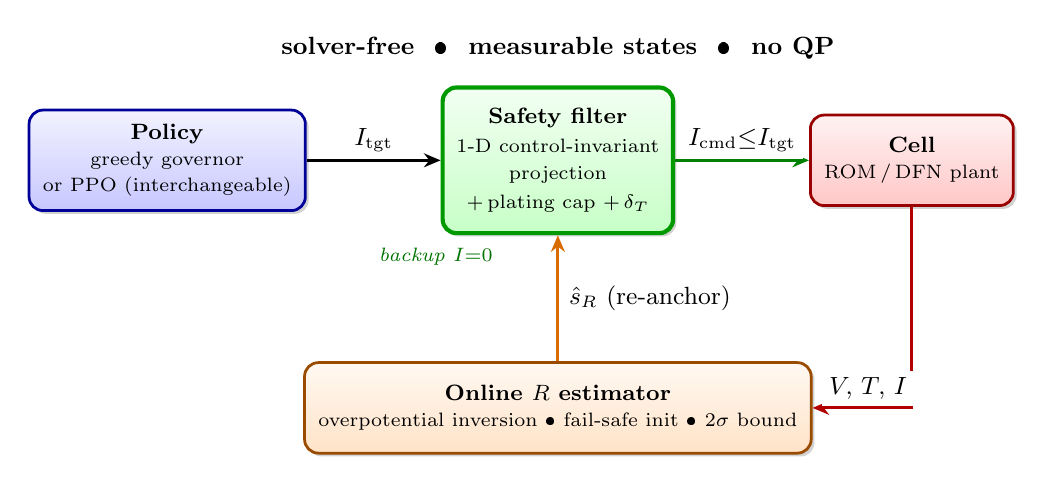
\begin{tikzpicture}[
 font=\footnotesize, node distance=0pt,
 >={Stealth[length=6pt,width=5pt]},
 blk/.style={rectangle, rounded corners=5pt, draw=#1!60!black, line width=1pt,
 top color=#1!5, bottom color=#1!22, align=center, text=black,
 minimum height=1.15cm, minimum width=2.35cm, inner sep=5pt,
 drop shadow={shadow xshift=1.2pt, shadow yshift=-1.2pt, opacity=0.32, fill=black!55}},
 sig/.style={font=\small, inner sep=2.5pt, fill=white, text=black},
]
\node[blk=blue] (pol) {\textbf{Policy}\\{\scriptsize greedy governor}\\{\scriptsize or PPO (interchangeable)}};
\node[blk=green, line width=1.5pt, minimum height=1.85cm, minimum width=2.9cm,
 right=1.7cm of pol] (fil) {\textbf{Safety filter}\\[1pt]{\scriptsize 1-D control-invariant}\\{\scriptsize projection}\\[1pt]{\scriptsize $+$\,plating cap\ $+$\,$\delta_T$}};
\node[blk=red, right=1.7cm of fil] (cell){\textbf{Cell}\\{\scriptsize ROM\,/\,DFN plant}};
\node[blk=orange, minimum width=6.0cm, below=1.6cm of fil] (est)
 {\textbf{Online $R$ estimator}\\{\scriptsize overpotential inversion \textbullet\ fail-safe init \textbullet\ $2\sigma$ bound}};
\draw[->,line width=1.1pt] (pol) -- node[sig,above]{$I_\mathrm{tgt}$} (fil);
\draw[->,line width=1.3pt,green!50!black] (fil) -- node[sig,above]{$I_\mathrm{cmd}{\le}I_\mathrm{tgt}$} (cell);
\draw[->,line width=1.1pt,red!70!black] (cell.south) |- (est.east) node[sig,pos=0.72,above]{$V,\,T,\,I$};
\draw[->,line width=1.1pt,orange!85!black] (est.north) -- node[sig,right=1pt]{$\hat s_R$\ (re-anchor)} (fil.south);
\node[font=\scriptsize\itshape, green!45!black, below=1pt of fil.south, xshift=-1.55cm] {backup $I{=}0$};
\node[above=6pt of fil.north, font=\small\bfseries]
 {\,solver-free \ \textbullet\ \ measurable states \ \textbullet\ \ no QP\,};
\end{tikzpicture}}
\caption{Control architecture. The policy proposes a target current, the safety filter projects it
to the largest value that keeps the one-step transition inside the safe set, and the online
estimator re-anchors the filter to the aging cell. Only the filter carries safety.}
\label{fig:arch}\end{figure}

\section{Related Work}
\textbf{Safe reinforcement learning} enforces constraints through soft penalties
\cite{iecon2022penalty}, Lagrangian relaxation \cite{stooke2020pid,achiam2017cpo}, action shielding
\cite{alshiekh2018shielding}, and learned safety layers \cite{cao2025adaptive,dalal2018safe}, each
supplying a statistical guarantee fitted to fresh dynamics; charging applications follow the same
pattern \cite{wei2022ddpg,kim2020rl,attia2020}. \textbf{Safety filters} certify or repair a proposed
input against a control-invariant set \cite{blanchini2008settheoretic}: control barrier functions
\cite{ames2019cbf}, reference governors \cite{gilbert2002governor}, Hamilton--Jacobi reachability
\cite{bansal2017hj}, and the predictive safety filter \cite{wabersich2021psf}. We specialize the last
to battery charging, where a trivial backup collapses it to a scalar projection. \textbf{Charging
controllers} span CC--CV, multi-stage CC, model predictive control, and Pontryagin-based optimal
profiles \cite{pmp2021,moura2017}; the model-based methods minimize loss directly but need an
accurate online model that aging erodes \cite{plett2015,waag2014}. No prior charging method combines
hard $T$/$V$ limits, an enforced plating constraint \cite{yang2017plating,arora1998}, resilience to
aging \cite{kirkaldy2024}, freedom from an SOH oracle, and real-time operation.

\section{Problem Formulation}
We charge a single LG~M50 cell (NMC811/graphite-SiOx, \SI{5}{Ah}), parameterized by the electro-thermal set of
Chen et al.\ \cite{chen2020} and the degradation set of O'Kane et al.\ (SEI plus partially
reversible plating) \cite{okane2022}, from 10\% to 80\% SOC within \SI{40}{min} from initial
temperature $T_0$, warm ($\SI{25}{\degreeCelsius}$, thermally limited) and cold
($\SI{10}{\degreeCelsius}$, plating limited). The \emph{guaranteed} safe set is
\begin{equation}
\mathcal{S}=\{\,T\le T_{\max},\ V\le V_{\max}\,\},\quad T_{\max}=\SI{45}{\degreeCelsius},\
V_{\max}=\SI{4.2}{V}.
\end{equation}
Here $T$ is the volume-averaged cell temperature both the ROM and the DFN report. Both constraints are \emph{instantaneously stoppable}, since
zero current halts heat generation and drops $V$ to the open-circuit voltage, which makes the
control-invariance argument below exact for them in the ROM. We also \emph{monitor} the plating
overpotential $\phi_{\mathrm{an}}=\phi_s-\phi_e$ at the separator interface ($\phi_{\mathrm{an}}<0$
signals plating) \cite{yang2017plating}, but plating is history-dependent and not
stoppable, so no one-step margin certifies it. We instead enforce a temperature-dependent current
cap, keeping $\mathcal S$ certified and plating only empirically enforced.

The state $x=(\text{SOC},T,V,I_\mathrm{prev},t/D,T_\mathrm{amb})$ uses measurable signals only, the
action is the target current $I\in[0,I_{\max}]$ under a slew-rate limit, the reward pays for charge net
of wall-energy loss, and the cost is constraint exceedance, a CMDP \cite{altman1999constrained}.

\section{Method}
\subsection{Solver-free control-invariant projection}
From the current state $x$, let $g(s_R,I)$ be the one-step reduced-order-model (ROM) prediction
of $(T,V,\phi_\mathrm{an})$ under resistance scale $s_R$ and applied current $I$. The filter
projects the policy's proposed current $I_\pi$ onto the largest admissible value,
\begin{equation}
I_\mathrm{cmd}=\max\{\,I\in[0,I_\pi]:g(s_R,I)\in\mathcal S_{-\delta}\,\},
\end{equation}
where $\mathcal S_{-\delta}$ tightens $\mathcal S$ by control margins $\delta$. Each constraint
is monotone in $I$, which makes the feasible set an interval $[0,I^\star]$ (Fig.~\ref{fig:proj}).
Bisection then finds $I^\star$ in $O(\log 1/\epsilon)$ model evaluations, with no matrix solve or
rollout.

\begin{figure}[tbp]\centering
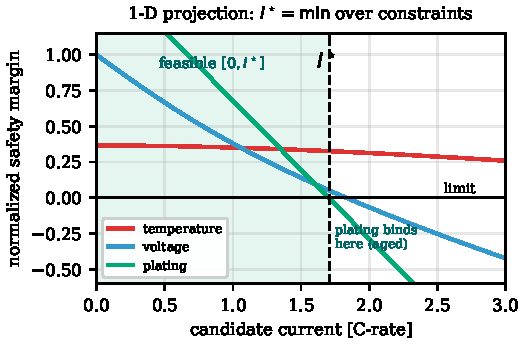
\includegraphics[width=\columnwidth]{fig_proj}
\caption{The solver-free projection. Each hard constraint is monotone in the applied current, so the
admissible set is a single interval and the certified cap is $I^\star=\min$ over the per-constraint
roots, found by bisection with no QP.}
\label{fig:proj}\end{figure}

\begin{proposition}[One-step control invariance in the ROM, up to $\delta_T$]\label{prop:inv}
For a control step $\Delta t\gtrsim\tau_\mathrm{RC}$, the input $I=0$ makes the input-driven heat
vanish and drops $V$ toward the OCV, leaving only a decaying RC residual bounded by
$e^{-\Delta t/\tau_\mathrm{RC}}$ that the margin $\delta_T$ absorbs. Thus $I=0$ is a feasible backup
and $\mathcal S$ is control-invariant in the ROM \emph{up to} $\delta_T$. That is, if
$x_0\in\mathcal S_{-\delta}$ and every step keeps the predicted $(T,V)\in\mathcal S_{-\delta}$, then
$x_t\in\mathcal S$ for all $t$. The invariance is thus margin-absorbed, not unconditional, and DFN
replay verifies the margin end to end.
\end{proposition}
\begin{proof}
At $I=0$ every input heat source vanishes and the lone RC residual $V_1^2/R_1$ decays by
$e^{-\Delta t/\tau_\mathrm{RC}}{\approx}0.37$ per step, bounded by $\delta_T$. With Newtonian cooling
$\dot T\le0$ up to $\delta_T$ whenever $T\ge T_\mathrm{amb}$ and $V\to\mathrm{OCV}\le V_{\max}$, the
input $I=0$ is a feasible backup at every $x_t\in\mathcal S$. The filter admits $I_\mathrm{cmd}$ only
when the one-step prediction lies in $\mathcal S_{-\delta}\subseteq\mathcal S$, so
$x_t\in\mathcal S$ for all $t$ by induction.\footnote{An extended version gives the step-size
derivation, the full margin derivation, and figure galleries.}
\end{proof}

Our step ($\Delta t=\tau_\mathrm{RC}=\SI{30}{s}$) meets the condition at one time constant, leaving
$\sim0.37$ of the RC overpotential energy after the cut, which the margin $\delta_T$ (base
\SI{0.5}{\degreeCelsius} plus a $\sim$\SI{4.25}{\degreeCelsius} cooling reserve) absorbs, with the
step-size tradeoff and residual bound detailed in the extended version. The invariance is exact in the
\emph{ROM}, and transfer to the DFN plant is bounded by the margins and confirmed by replay
(Sec.~\ref{sec:results}), not asserted, while the plating potential, carrying diffusion
memory, stays excluded from $\mathcal S$ and enforced empirically.

We keep ``certified'' scoped to what it proves: exactly one theorem, in the lumped ROM, on
volume-averaged temperature, through the high-current phase where $\hat s_R\ge s_R^\star$ is pinned.
Everything else is simulation-validated with one-sided Clopper--Pearson bounds.

\subsection{Plating as a monotone constraint}
The anode overpotential is affine and decreasing in current, so plating enters the same monotone
bisection as $T$ and $V$ with a certified cap wherever a nonnegative one exists. The $I{=}0$ backup,
however, does not clear the plating margin at the cold, aged, high-SOC corner, so plating is not
control-invariant on its own. We keep the trajectory feasible with a temperature-dependent current cap
(\SI{2}{C} at $\SI{25}{\degreeCelsius}$ tapering to \SI{1.0}{C} at $\SI{10}{\degreeCelsius}$, fit from
closed-loop DFN residuals) and monitor it without claiming a guarantee.

\subsection{Aging without an oracle, and why a bound is enough}
\label{sec:method-aging}
Internal resistance grows with age \cite{kirkaldy2024}, and a filter anchored to fresh
dynamics under-predicts heat and voltage and turns unsafe. We estimate the resistance scale $\hat s_R$
online by inverting the measured overpotential \cite{plett2015,waag2014} and re-anchor the certificate
every step, offsetting the thermal margin by the estimate. The estimator is \emph{fail-safe}: it
initializes worst-case and relaxes toward the measurement, staying conservative from step one on the
same noisy sensors the policy reads. Its job is far weaker than identification, since resistance enters
heat and voltage monotonically and a larger scale only makes the filter more cautious.

\begin{proposition}[Monotone safety in the aging channels]\label{prop:mono}
Let aging act through two scalar channels. A resistance scale $s_R$ multiplies the ohmic heat
and voltage rise, and a cooling-loss factor $\gamma\ge1$ divides the effective heat-transfer
coefficient, so the temperature rise scales with $\gamma$. For the certified set
$\mathcal S=\{T\le T_{\max},V\le V_{\max}\}$, each one-step peak $g_c(s_R,\gamma,I)$,
$c\in\{T,V\}$, is non-decreasing in the current $I$ and in \emph{each} channel $s_R,\gamma$, so
the certified cap $I^\star(s_R,\gamma)$ is non-increasing in each. Hence for a plant with true
channels $(s_R^\star,\gamma^\star)$, any $(\hat s_R,\hat\gamma)\succeq(s_R^\star,\gamma^\star)$
commands a current the plant already admits. Oracle-free safety on $\mathcal S$ therefore needs
only a conservative \emph{bound on each channel}, never the exact values.
\end{proposition}
\begin{proof}
The thermal map is $T'{=}T{+}\tfrac{\Delta t}{C_\mathrm{th}}(Q_\mathrm{gen}{-}\tfrac{hA}{\gamma}(T{-}T_\mathrm{amb}))$
with generation $Q_\mathrm{gen}{=}I^2R_\Omega s_R{+}Q_\mathrm{act}(I){+}Q_\mathrm{rev}$, and the terminal
voltage is $V{=}\mathrm{ocv}{+}IR_\Omega s_R{+}\eta_\mathrm{act}(I){+}V_1$, and three partial derivatives settle it.
Both $\partial_I g_T$ and $\partial_I g_V$ are non-negative, since the ohmic and activation terms rise
with current. Both $\partial_{s_R}g_T$ and $\partial_{s_R}g_V$ are non-negative, since the resistance
scale multiplies ohmic heat and voltage. And $\partial_\gamma g_T\ge0$ whenever $T\ge T_\mathrm{amb}$,
since worse cooling adds heat. The endothermic $Q_\mathrm{rev}{=}I\,T\,\mathrm dU/\mathrm dT$ stays below
$24\%$ of the irreversible heat and never overturns $\partial_I g_T\ge0$, verified numerically over $10$--$80\%$
SOC. Each $g_c$ is thus non-decreasing in $I$ and in each channel, so $I^\star$ is non-increasing in each,
and any $(\hat s_R,\hat\gamma)\succeq(s_R^\star,\gamma^\star)$ commands a current the plant admits.
\end{proof}
Reducing aging to these two channels drops nothing that matters, because capacity fade, OCV shift,
and entropic and diffusion terms need no margin, since the projection re-solves at the true state and the full-DFN ensemble
carries them, leaving only resistance and cooling to erode the $T$/$V$ headroom monotonically.

The fail-safe initialization supplies the bound, starting at $\hat s_R{=}1.8$, the rated
end-of-life resistance from the datasheet aging envelope, a fixed design constant known before
deployment, not a per-cell oracle, so $\hat s_R\ge s_R^\star$ holds from step one across the
rated range and meets Prop.~\ref{prop:mono}'s precondition by construction. A cell aged \emph{past}
rated end of life ($s_R^\star>1.8$) falls outside it, exactly where a BMS should retire the cell. A
higher assumed scale only throttles harder and delivers less charge, so the estimator is
\emph{safety-neutral}. By Prop.~\ref{prop:inv} any policy the filter projects stays safe, and the
estimate's error costs SOC, never a violation.

The margin realizes both channels of Prop.~\ref{prop:mono},
$\delta_T{=}\delta_{T0}{+}K(\hat s_R{-}1){+}f(T{-}T_\mathrm{amb})$. The throttle ($K{=}15$) converts
the resistance bound into thermal headroom, and the reserve ($f{=}0.25$) holds back a fraction $f$ of
the temperature rise, certifying any cooling loss up to $\hat\gamma{=}1{+}f$, a $20\%$ fault. The
gains are sized to that $20\%$-loss edge, not fitted to a failure. Sweeping them over $K\in[5,25]$ and
$f\in[0.1,0.4]$ leaves zero violations in every cell of the aged, cooling-faulted grid, a safe region, not a tuned point. The reserve also proves conservative, holding safety to a $\coolSafeLoss\%$
cooling loss where it certifies $20\%$. We freeze the gains and test on a \emph{disjoint} ensemble they never saw, and the filter stays safe on
every held-out draw, including the joint noise/aging/out-of-model case a real BMS faces
(Sec.~\ref{sec:results}, Table~\ref{tab:safety}).

The margin's price is aged charge. With the estimator in the loop, delivered SOC falls from
\estSocFresh\ fresh to \estSocAged\ at SOH~0.8 at zero violations; a non-adaptive filter keeps
delivering \estNomSocAged\ but violates $T$/$V$. Closing the loop against the DFN, the SOH~0.8 cell
reaches \clSocAged\ SOC within $3$ points of the in-model value, ruling out a ROM artifact. The conservative bound alone gives a \clOracleSocAged\ floor, plus the estimator's $\sim$\SI{3}{\%}. At
rated end-of-life the filter trades roughly a quarter of fresh SOC for the margin.

\subsection{Policy as a control, not a claim}
Because the filter carries safety for \emph{any} input, the policy is free. Its deployable default is a
greedy governor requesting $I_{\max}$ every step. A PID-Lagrangian PPO actor--critic
\cite{schulman2017ppo,stooke2020pid} trained with the projection active is indistinguishable from it
(Sec.~\ref{sec:results}). We therefore treat the governor as the method and PPO as an ablation.

\section{Experimental Setup}
The filter runs on a lumped ROM with three coupled parts \cite{newman2004}. A single-RC branch carries
a temperature-dependent ohmic resistance, a lumped thermal state absorbs the ohmic, reaction, and
reversible heat \cite{bernardi1985}, and a surrogate tracks the plating overpotential
\cite{yang2017plating}. Its parameters are fit to the Doyle--Fuller--Newman model
\cite{doyle1993,fuller1994} under the parameterization of O'Kane et al.\ \cite{okane2022} by simulated charging
sweeps with a held-out split (voltage RMSE
\VRMSE~mV, held-out \VRMSEho~mV, temperature RMSE \TRMSE~\degC).
Every
safety claim is then validated out of sample by replaying the \emph{realized} current in the full DFN
in PyBaMM \cite{sulzer2021pybamm}, so the ROM never self-reports safety, and worst-case out-of-distribution excursions are disclosed below.

We compare CC--CV at several rates, multi-stage CC (MSCC), an offline time-optimal profile, a
filter-free PID-Lagrangian PPO, and our filtered policy, all learned methods sharing the MDP,
network, and budget. Metrics are system efficiency $\eta_\mathrm{sys}$ (cell energy over wall energy,
including converter loss), delivered SOC at the deadline, DFN peak temperature, and the
any-constraint violation rate over $n$ episodes, reported with a Clopper--Pearson $95\%$ upper bound
\cite{clopper1934}.
The main aging comparison counts $n{=}30$ distinct scenarios, an honest rule-of-three bound of $10\%$,
while the held-out ensembles use larger $n$.

\section{Results}\label{sec:results}
\subsection{Main comparison}
Table~\ref{tab:main} gives the warm comparison; the peak is DFN-replayed, and the violation column pairs
each baseline's observed any-constraint rate with a $T$/$V$-only Clopper--Pearson bound for ours. Fast
CC--CV and MSCC hit the target SOC but
overshoot \SI{45}{\degreeCelsius} in every episode. Conservative CC--CV 1C stays thermally cool
(peak \SI{38.7}{\degreeCelsius}) yet still \emph{plates} in 22\% of episodes (all its violations
are plating, none thermal), a reminder that even a moderate sustained rate drives the anode
negative at high SOC. Our filtered
policy holds zero observed thermal and voltage violations (Clopper--Pearson upper bound
$\le$\oursWarmUpper\%). It matches CC--CV~1C's SOC while removing that protocol's $22\%$ plating (Fig.~\ref{fig:pareto}). A \emph{predictive} controller banks more with foresight, the offline optimum
reaching \SI{0.798}{} by seeing the future and a causal MPC banking more at the cost of an online
solver (Sec.~\ref{sec:solver}). The filter also keeps headroom, sitting near \SI{40.7}{\degreeCelsius}, the \SI{45}{\degreeCelsius} limit \emph{less} its cooling-robustness
margin, so a cooling fault keeps slack; the offline optimum reserves none and rides to
\SI{44.5}{\degreeCelsius}. The filter-free PID-Lagrangian PPO \cite{stooke2020pid} delivers less charge
(\SI{0.734}{}) and still violates $9\%$, the soft-penalty hedge the hard filter avoids.

\begin{figure}[tbp]\centering
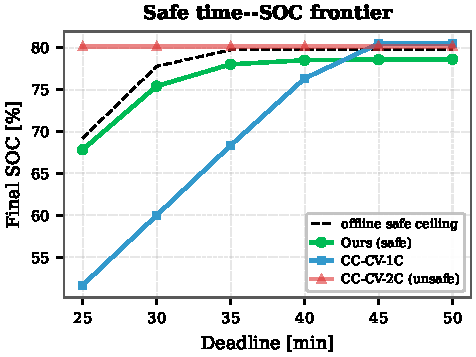
\includegraphics[width=\columnwidth]{fig5_pareto}
\caption{Safe time--SOC frontier. Delivered SOC against the charge deadline at zero observed thermal
or voltage violations. Our filter sits on the safe frontier, trailing only the non-causal offline
optimum that reserves no cooling margin.}
\label{fig:pareto}\end{figure}


\begin{table}[t]
\caption{Warm comparison at $\SI{25}{\degreeCelsius}$ over $40$ frozen CRN conditions.}
\label{tab:main}
\centering\footnotesize
\begin{tabular}{lcccc}\hline
Method & $\eta_\mathrm{sys}$[\%] & SOC & $T_\mathrm{pk}$[\degC] & Viol.[\%]\\\hline
\iecomainrows\hline
\end{tabular}
\end{table}

The binding constraint flips with temperature. Warm, temperature binds and plating is slack. Cold
(\SI{10}{\degreeCelsius}), the anode overpotential binds first and the plating cap tapers to
\SI{1.0}{C}, and the same filter handles both without retuning since the projection reads whichever
constraint is closest. Cold is the harder regime, where our filter delivers \oursColdSoc\ SOC at
zero violations while both CC--CV rates violate and the causal gap widens from \SI{3.0}{\%} warm to
\SI{9.1}{\%} cold.

Table~\ref{tab:causal} shows the payoff of a policy-agnostic guarantee. The greedy governor and the
trained PPO policy deliver the same SOC, peak, and violation rate, because the filter, not the
policy, sets the operating point, so the simplest policy suffices and no learning is needed for
safety. The governor is not globally optimal; the non-causal offline optimum banks \SI{3.0}{\%} more
SOC by easing early with foresight.
So across warm and cold the filter is the charge-maximal deployable choice at zero observed violations,
and only an online solver or non-causal foresight does better.

\begin{table}[t]
\caption{Causal optimality, DFN-replayed (warm, fresh).}
\label{tab:causal}
\centering\footnotesize
\begin{tabular}{lcccc}\hline
Method & SOC & $T_\mathrm{pk}$[\degC] & Anode[mV] & DFN-safe\\\hline
\causalrows\hline
\end{tabular}
\end{table}

\subsection{Safety under aging, without a health oracle}
On cells aged to SOH~$\{1.0,\dots,0.8\}$, the filter with the true aged model holds violations at
0\%, while without adaptation it rises to \agingFixnomViol\% at SOH~0.8 and a filter-free
PPO-Lagrangian to \agingPPOLagViol\% (Fig.~\ref{fig:aging}), the non-adaptive filter eroding its own
thermal certificate as the cell ages. Closing the loop without an oracle,
our online estimator holds violations at \estViolMax\% across the SOH range, \estViolNoise\% under
sensor noise, where the non-adaptive filter fails \nomAgedViol\%. The aged-thermal margin is
empirical out of model, so we test it statistically, and on a disjoint held-out ensemble it is safe
on \valSafe/\valN\ draws (worst \valWorstT~\degC, bound \valCP\%) where the non-adaptive filter
overheats. Table~\ref{tab:safety} collects every $T$/$V$ stress test with its bound, including the
joint case (noise, aging, and out-of-model DFN, bound \jointCP\% at $n{=}\jointNbig$) and the
cross-chemistry recalibration; each row counts violations over independent aged-DFN draws with the
gains frozen, not i.i.d.\ cells. Safety thus holds across the rated aging range with no per-cell
identification, the deployment property fresh-cell validation can never establish.

\begin{table}[t]
\caption{All $T$/$V$ safety evidence by stress test, with sample size, violations, and a one-sided
Clopper--Pearson $95\%$ upper bound.}
\label{tab:safety}
\centering\footnotesize
\begin{tabular}{lccc}\hline
Stress test & $n$ & viol.\ & CP $95\%$ [\%]\\\hline
\safetytablerows\hline
\end{tabular}
\end{table}

\begin{figure}[tbp]\centering
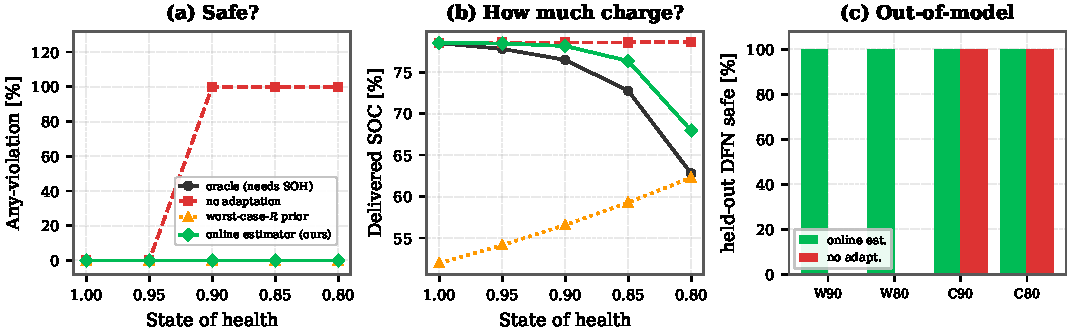
\includegraphics[width=\columnwidth]{fig3_aging}
\caption{Deployment across the SOH range. \textbf{(a)}~among the filtered variants, only ``no
adaptation'' violates, and early
($100\%$ of episodes from SOH~0.9). Oracle, worst-case-$R$ prior, and our estimator
stay at 0\% in model. \textbf{(b)}~the worst-case prior wastes charge on healthy cells while the
estimator recovers the oracle's charge. \textbf{(c)}~held-out aged-DFN ensemble, where the estimator
stays safe out of model.}
\label{fig:aging}\end{figure}

\subsection{Safety needs a bound, not identification}
Fig.~\ref{fig:mono} closes the entire loop against the DFN and sweeps the resistance scale fed to
the filter. The closed-loop \emph{peak} temperature inherits Prop.~\ref{prop:mono}'s monotonicity,
falling from \SI{45.1}{\degreeCelsius} at $\hat s_R{=}1.0$ to \SI{26.9}{\degreeCelsius} at
$\hat s_R{=}2.2$ (SOH~0.8), and the safe boundary sits near $\hat s_R{\approx}1.1$, far below the
true $s_R^\star{=}1.8$. The fail-safe init thus clears it with room to spare, so oracle-free safety
rests on the bound, not on the DFN matching the ROM, and the resistance estimator sets only
charge speed. The one orthogonal fault, an unmodeled cooling loss, is handled by the margin's second
channel.

\begin{figure}[tbp]\centering
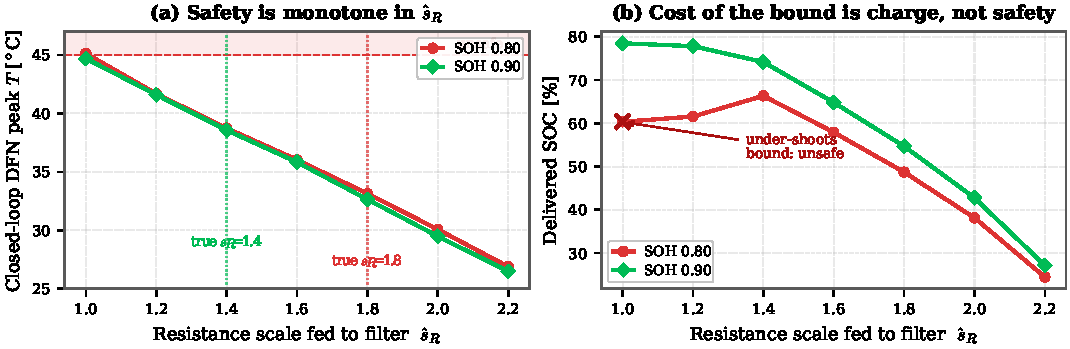
\includegraphics[width=\columnwidth]{fig10_monotone}
\caption{Closed-loop against the DFN, safety is monotone in the resistance scale the filter is
told to use (Prop.~\ref{prop:mono}). \textbf{(a)}~peak temperature falls as $\hat s_R$ grows.
Every value past a boundary near $1.1$, well below the true aged $s_R^\star$ (dotted), is safe,
so a conservative bound certifies safety without identifying $s_R^\star$.
\textbf{(b)}~the bound's only price is delivered charge, which is why an online estimate still
earns its keep, for speed. Under-shooting the bound ($\hat s_R{=}1.0$, $\times$) is the lone
unsafe point.}
\label{fig:mono}\end{figure}

The estimate \emph{under}-shoots by end of charge ($\hat s_R{\to}\clRestAged$ vs
$s_R^\star{=}\clRtrueAged$), which would be unsafe were the final estimate the certificate. It is
not, because the fail-safe init pins $\hat s_R{=}1.8\ge s_R^\star$ through the high-current phase and
the dip below $s_R^\star$ comes only at \precondDipMin~min, once current has fallen to \precondDipI~C
with the cell \precondDipHead~\degC below the limit. The theorem carries the stressful phase, the
margin the tail, and the estimate's error costs charge, never safety.

\subsection{High-fidelity DFN validation}
\label{sec:dfn}
On the plating channel, our nominal warm and cold profiles hold minimum anode potentials of
$+\dfnOursWarmSurf$~mV and $+\dfnOursColdSurf$~mV, both positive, where CC--CV~2C drives the cold
anode to $\dfnCctwoColdSurf$~mV. Under an adversarial out-of-distribution ensemble that breaks the plating calibration, the cap holds
on \oodWarmSafe/\oodWarmN\ warm and \oodColdSafe/\oodColdN\ cold draws (worst \oodWorst~mV, cold
bound \oodColdCP\%), the few breaches landing in the cold corner the monotonicity flags.

The certified margin is not an artifact of the reference degradation set \cite{okane2022}. Replaying our aged profiles across a perturbed
Chen et al.\ ensemble (same \SI{4.2}{V}/\SI{5}{Ah} spec) holds $T$/$V$ on all
\crossEnsSafe/\crossEnsN\ draws (bound \crossEnsCP\%); recalibrating the \emph{entire} ROM (OCV,
overpotential, thermal) to the Enertech cell of Ai et al.\ \cite{ai2020} (\SI{\chemTwoQ}{Ah}, a different manufacturer,
voltage RMSE \chemTwoV~mV) keeps the closed-loop filter safe on all \chemTwoSafe/\chemTwoN\ aged draws
(bound \chemTwoCP\%, Table~\ref{tab:safety}). That cell runs cool (peak \SI{28}{\degreeCelsius}), so
voltage binds and the test exercises the \emph{voltage} certificate's transfer. Plating recalibration
would need kinetics that set lacks, so it stays LG~M50, and hardware remains out of scope. The
certificate therefore survives high-fidelity electrochemistry and a change of chemistry, evidence that
safety follows from the method and not a tuned parameter set.

\subsection{Solver-free feasibility versus MPC}\label{sec:solver}
The projection is the only online computation carrying safety, a bisection of a few ROM forward maps
with no matrix factorization. Its safety logic is \filterSloc\ numpy-only source lines a
functional-safety audit can read in full, where an embedded QP instead places a compiled ADMM solver
(\qpTcbFiles\ bundled C files) in the trusted computing base. Against a receding-horizon MPC ladder,
nominal MPC (fresh $R$) violates \mpcNomViol\% under aging, while an MPC given the \emph{same}
fail-safe bound is oracle-free and safe (\mpcBoundedViol\%), as is an oracle MPC (\mpcOracleViol\%).
Oracle-freedom is thus Prop.~\ref{prop:mono}'s doing, shared by any bounded controller, not the
filter's. Unique to the filter is Prop.~\ref{prop:inv}, replacing the solver with a fixed
$18$-iteration bisection of the \emph{exact} constraint, ceding some charge to the foresighted MPC
(\mpcOursSoc\ vs \mpcBoundedSoc) for that simplicity. The trade is deliberate, buying MPC-class safety
without a solver in the trusted computing base for a few points of charge.

\section{Conclusion}
We built a real-time safety filter for fast charging that needs no online solver and no state-of-health
oracle, and two facts carry it. Zero current is a universal safe backup for temperature and voltage,
collapsing the predictive safety filter to a scalar bisection. Safety is monotone in the two aging
channels, resistance growth and cooling loss, so a conservative datasheet bound certifies it and no
parameter is identified. The bound carries safety, and the online estimator only buys charge speed.

The filter records zero observed temperature and voltage violations over
hundreds of DFN-confirmed episodes where fast CC--CV overshoots \SI{45}{\degreeCelsius} every time.
It stays safe on \valSafe/\valN\ disjoint aged draws (Clopper--Pearson bound \valCP\%) and under a full
recalibration of the ROM to a second cell chemistry, so the guarantee is a property of the method and
not one cell. It delivers the charge of CC--CV at 1C while removing that protocol's plating, and a
trivial greedy governor matches a trained RL policy on every metric, which isolates the filter as the
safety carrier. The certified path is \filterSloc\ numpy-only source lines, small enough to audit.

The certificate is ROM-relative on volume-averaged temperature, the
evidence is simulation over an aged-DFN distribution and not a hardware rating, and plating is enforced
and monitored, not certified. Hardware validation, a predictive plating constraint, an age-aware cap,
and a pack-level extension are the natural next steps. We release the filter, ROM, executable
proposition checks, and a one-command reproduction as an MIT-licensed reference implementation at
\url{https://github.com/keshavkrishnan08/safe-charge}.

\bibliographystyle{IEEEtran}
\bibliography{refs}
\end{document}
